\section{Технологический раздел}\label{sec:technic}
\subsection{Сборка компилятора}
Компилятор написан на языке Python версии 3.10, поэтому может быть запущен на любой операционной системе, имеющей
компилятор этой версии языка Python.

Перед запуском компилятора необходимо установить необходимые зависимости: скачать и собрать LLVM,
установить необходимые библиотеки командой:
\begin{lstlisting}[language=bash,caption={Установка зависимостей},label={lst:install}]
    pip3 install -r requirements.txt
\end{lstlisting}


\subsection{Запуск компилятора}\label{subsec:run}
Для запуска компилятора необходимо выполнить команду
\begin{lstlisting}[language=bash,caption={Установка зависимостей},label={lst:run}]
    python main.py main.go
\end{lstlisting}

В результате работы компилятора будет создан файл на языке LLVM IR output.ll, который необходимо скомпилировать для
текущей платформы:
\begin{lstlisting}[language=bash,caption={Установка зависимостей},label={lst:compile}]
    llc output.ll -fileType=obj -o output.o && gcc output.o
\end{lstlisting}

\subsection{Пример использования}
В качестве примера использования рассматривается код на языке Golang, который выводит в стандартный поток вывода числа от
0 до 10.

\begingroup
    \lstinputlisting[language=go,caption={Исходный код на языке Golang},label={lst:src}]{code/main.go}
\endgroup

Абстрактное синтаксическое дерево для данной программы представлено на рисунке~\ref{fig:tree}.
\begin{figure}[h!]
    \centering
    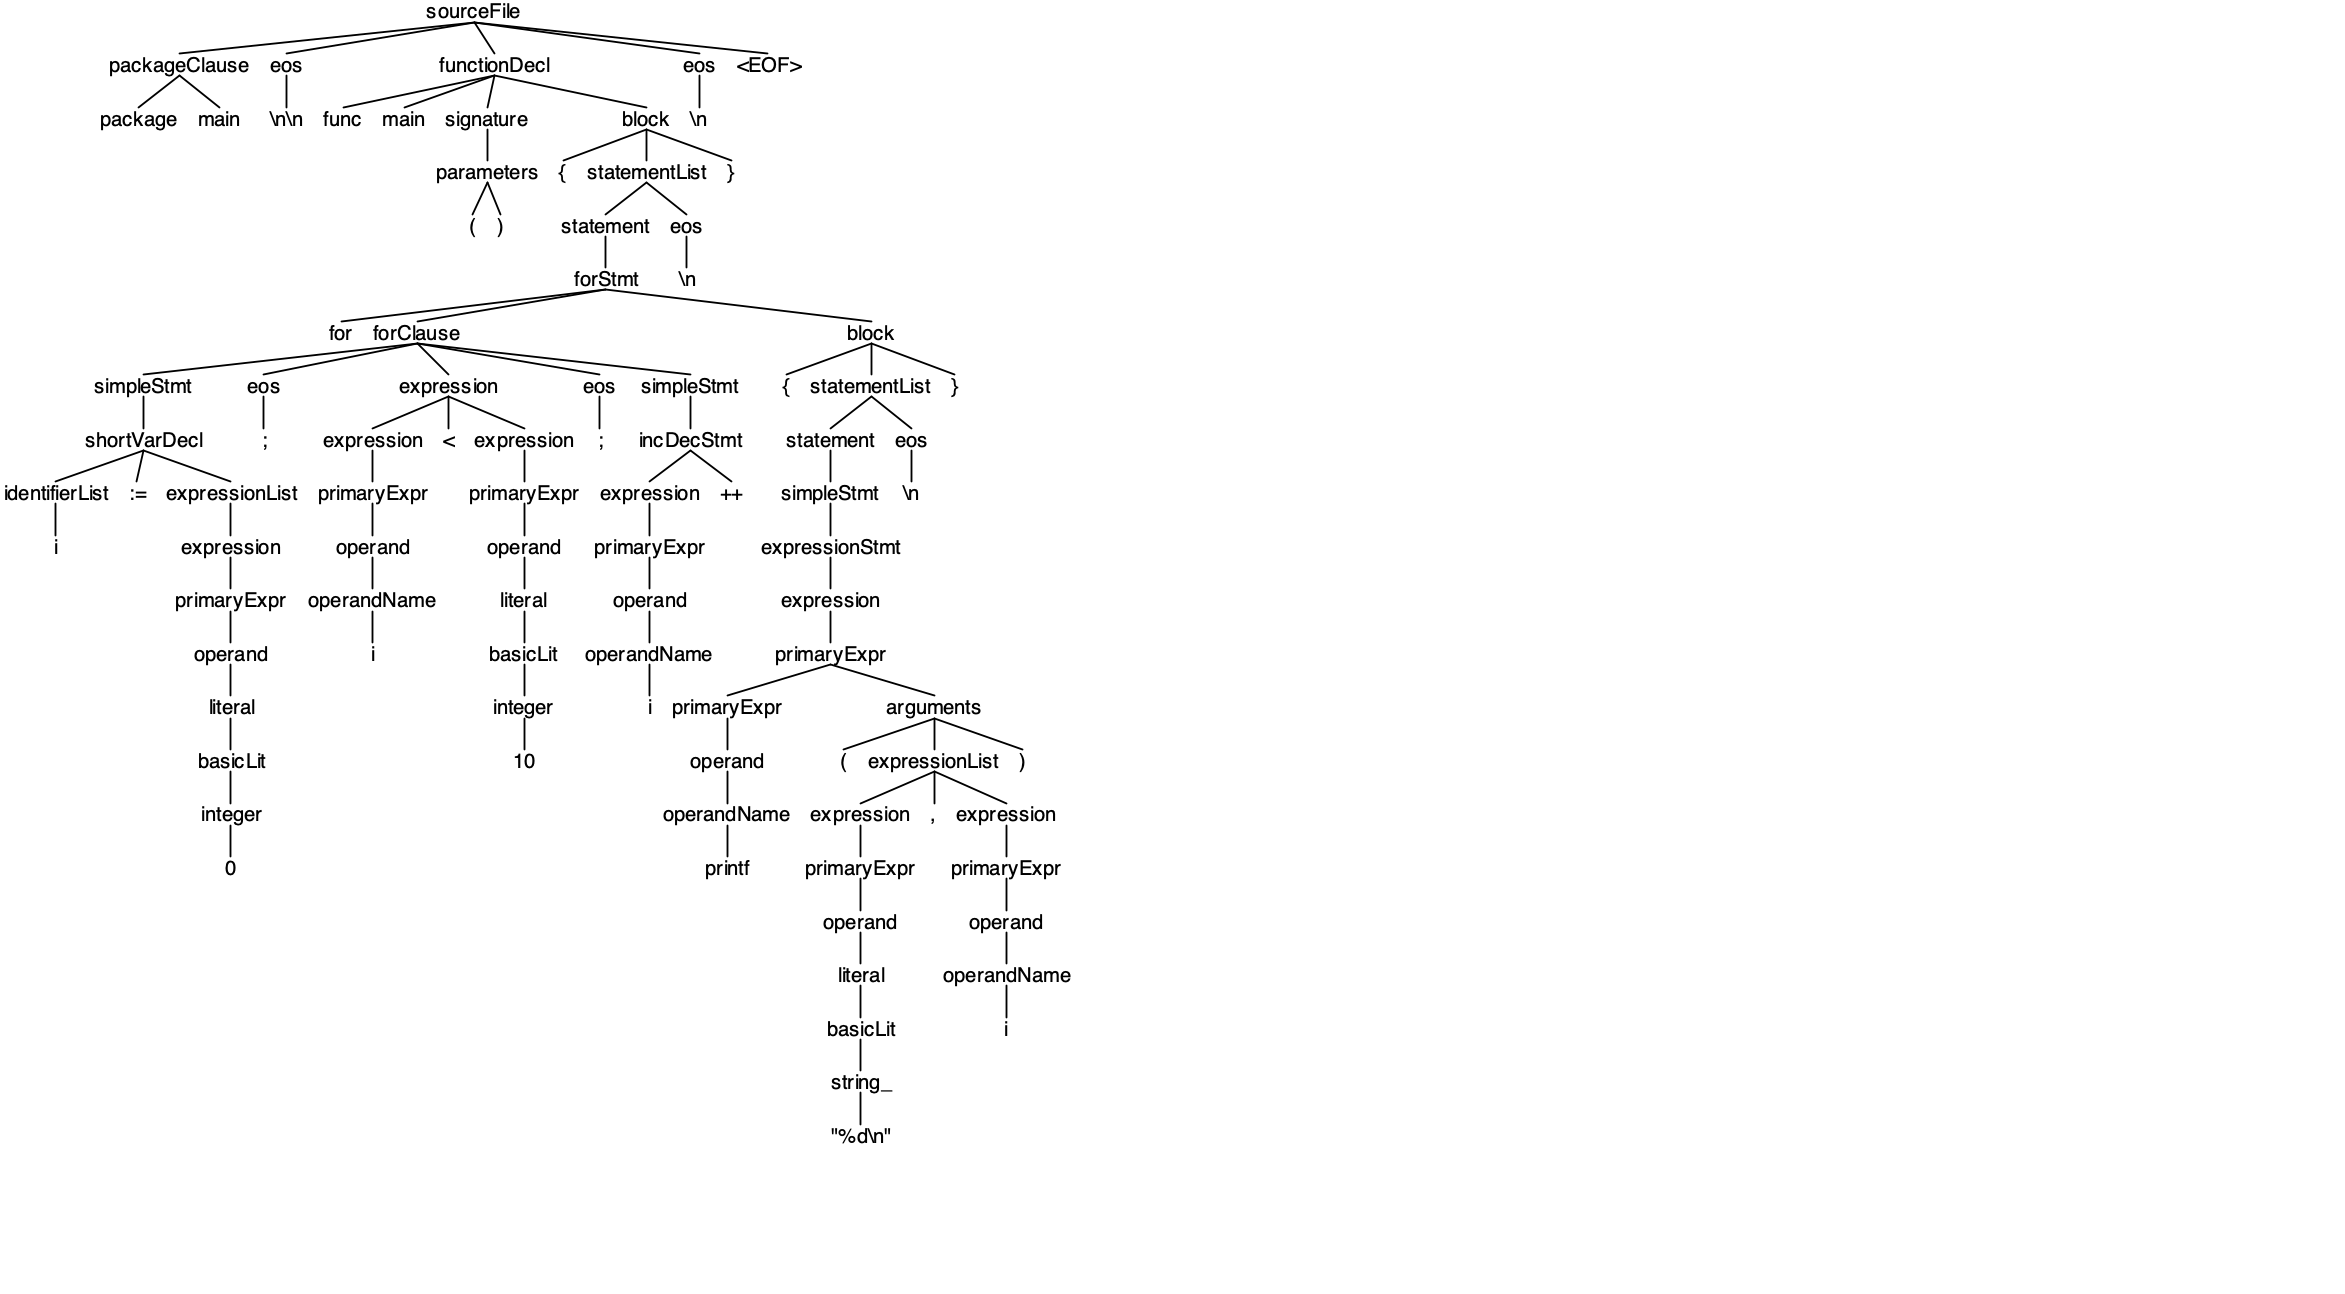
\includegraphics[scale=0.4]{img/tree}
    \caption{AST программы печати чисел от 0 до 10}
    \label{fig:tree}
\end{figure}

Результатом работы компилятора является код на языке промежуточного представляения LLVM IR, он представлен в
приложении В.

При запуске программы, в стандартный поток вывода печатаются числа от 0 до 10, рисунок~\ref{fig:print}
\begin{figure}[h!]
    \centering
    \fbox{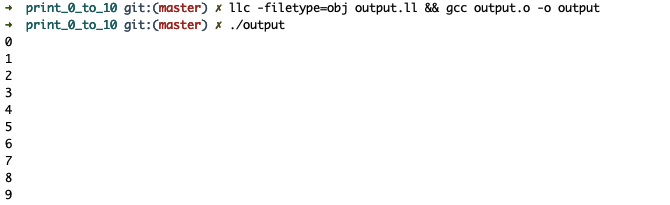
\includegraphics[scale=0.7]{img/print_0_to_10}}
    \caption{Вывод программы, печатающей символы от 0 до 10}
    \label{fig:print}
\end{figure}
